\documentclass[red]{beamer}
\setbeamertemplate{navigation symbols}{}
\usepackage[utf8x]{inputenc}
\usepackage{graphicx}
\usepackage{beamerthemeshadow}

\usetheme{CambridgeUS}
\setbeamercolor{itemize item}{fg=red} % all frames will have red bullets

\begin{document}
\title{Solving CAPTCHAs}
\author[MM, LM, SN, AS]{Mihai Maruseac, Lucian Mogoșanu, Sofia Neață, Adrian Șendroiu}
\date{March 2012}

\pgfdeclareimage{q}{img/q}

\maketitle

\begin{frame}{Admin}
  \begin{itemize}
    \item Team: UnCAPTCHA
      \begin{itemize}
        \item Mihai Maruseac
        \item Lucian Mogoșanu
        \item Sofia Neață
        \item Adrian Șendroiu
      \end{itemize}
    \item Repo: \url{https://github.com/mihaimaruseac/ssl}
  \end{itemize}
\end{frame}

\begin{frame}{Architecture - Overview}
  \begin{center}
    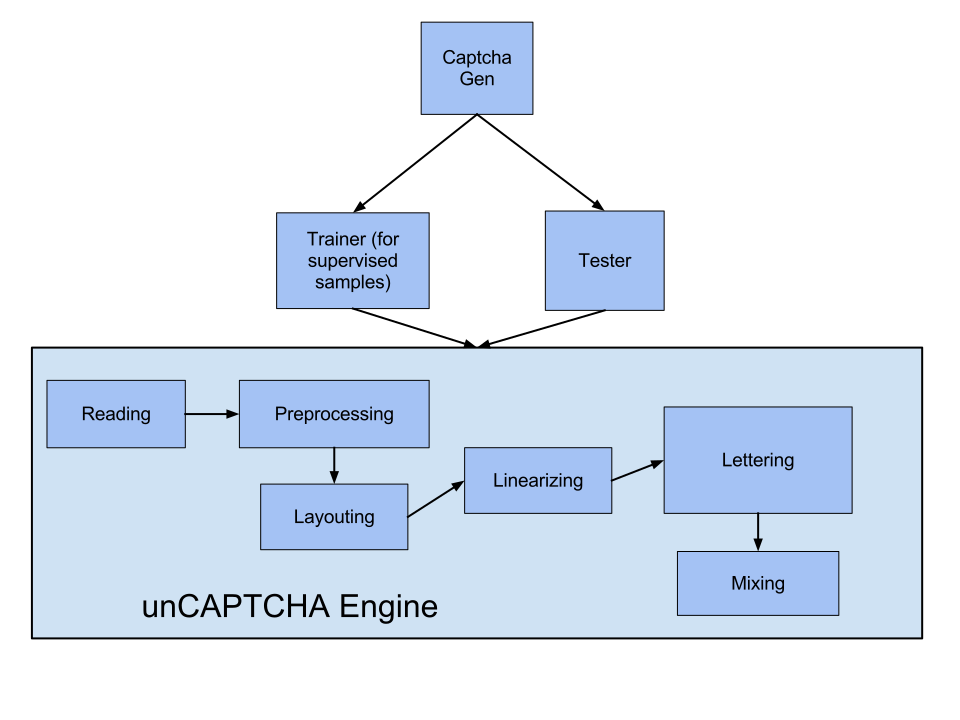
\includegraphics[width=0.85\textwidth]{img/unCAPTCHAarchitecturedraft.pdf}
  \end{center}
\end{frame}

\begin{frame}{CAPTCHA generation}
  \begin{itemize}
    \item Securimage
    \item PHP
    \item \texttt{show()} method of \texttt{Securimage()} class
    \item configurable parameters
  \end{itemize}
\end{frame}

\begin{frame}{CAPTCHA generation parameters}
  \begin{itemize}
    \item image size
    \item text perturbation
    \item text noise
    \item code length
    \item number of lines
    \item colour parameters: text, noise, background etc.
    \item optional custom background
  \end{itemize}
\end{frame}

\begin{frame}{CAPTCHA generation now}
  \begin{itemize}
    \item no distortions, noise or lines
    \item black on white text
  \end{itemize}
\end{frame}

\begin{frame}{CAPTCHA generation session}
  \begin{itemize}
    \item \texttt{supervised-gen.php}
    \item \texttt{supervised-get.php}
  \end{itemize}
\end{frame}

\begin{frame}{After CAPTCHA generation}
  \begin{itemize}
    \item use a set of scripts and C files to convert image to libSVM format
    \item \texttt{label index:val index:val index:val index:val}
    \item use libSVM to recognize letters
  \end{itemize}
\end{frame}

\begin{frame}{Thank you}
  \begin{center}
    \pgfuseimage{q}
  \end{center}
\end{frame}

\end{document}
